\section{Messungen und Auswertungen}
Bereits in der Projektarbeitsanfrage wurden konkrete Messungen für das fertige System vorgesehen. Diese betreffen einerseits die Stromversorgung und andererseits die Aktorik sowie die Rückführung über Encoder. Dieser Abschnitt dokumentiert die durchgeführten Messungen sowie deren Auswertung.

\subsection{Messungen an den Powerrails}
Die Stromversorgung ist ein zentrales Teilsystem der gesamten Platine. Deshalb wurden die einzelnen Versorgungsschienen nicht nur auf ihre Sollspannung, sondern auch auf ihr Verhalten unter Last untersucht. Im Vordergrund standen dabei Spannung und Strom unter Last, Leistungsaufnahme, Wirkungsgrad und Stabilität.

\subsubsection{Messaufbau}
Als Spannungsquelle wurde ein Labornetzteil mit einer Ausgangsspannung von 12V angeschlossen. 

Nach der Leerlaufmessung wurden die Powerrails gemeinsam belastet. Für die 6V Rails kam je eine Elektronische Last und für die 5V Rail der Raspberry Pi zum Einsatz.

Die 3,3-V-Logikversorgung wurde nicht als eigene Powerrail-Messung geführt, da sie aus der 5-V-Schiene abgeleitet wird.

Gemessen wurden:

\begin{itemize}
	\item Eingangsspannung und Eingangsstrom des Wandlers
	\item Ausgangsspannung und Ausgangsstrom der jeweiligen Schiene
	\item eventuelle Spannungseinbrüche beim Lastwechsel
	\item Schaltverhalten beim Ein- und Ausschalten
\end{itemize}

Die Messwerte wurden einheitlich in einer Tabelle erfasst. Die Spalte \glqq unter Last\grqq{} bezieht sich dabei auf die gemeinsame Belastung aller direkt genutzten Rails.

\begin{figure}[H]
	\centering
	\begin{tikzpicture}[font=\scriptsize, node distance=1.25cm, >=latex]
		\tikzstyle{block} = [draw, rectangle, rounded corners=2pt, minimum height=1.0cm, minimum width=2.3cm, align=center]
		\tikzstyle{meter} = [draw, circle, minimum size=0.75cm, align=center]
		\tikzstyle{line} = [draw, -latex']
		
		\node[block, fill=gray!15] (source) {Labornetzteil\\12 V / Anzeige};
		\node[block, fill=blue!12, right=of source] (board) {Controller-Board\\DC/DC-Wandler};
		\node[meter, fill=yellow!20, right=of board] (aout) {A};
		\node[block, fill=green!12, right=of aout] (load) {definierte Last\\oder Verbraucher};
		\node[above=0.28cm of source] {$U_\mathrm{in}$ / $I_\mathrm{in}$ am Netzteil};
		
		\path (aout) -- (load) coordinate[pos=0.5] (sense);
		\node[meter, fill=orange!18] (vout) at ([yshift=-0.8cm]sense) {V};
		\coordinate (gndL) at ([yshift=-1.55cm]source.south west);
		\coordinate (gndR) at ([yshift=-1.55cm]load.south east);
		
		\draw[line] (source) -- (board);
		\draw[line] (board) -- node[above] {6 V / 5 V} (aout);
		\draw[line] (aout) -- node[above] {$I_\mathrm{out}$} (load);
		\node[left=0.1cm of vout] {$U_\mathrm{out}$};
		\draw[draw] (sense) -- node[left] {} 	(vout.north);
		\draw[draw] (gndL) -- node[below] {GND} (gndR);
		\draw[draw] (source.south) -- (source.south |- gndL);
		\draw[draw] (board.south) -- (board.south |- gndL);
		\draw[draw] (load.south) -- (load.south |- gndL);
		\draw[draw] (vout.south) -- (vout.south |- gndL);
	\end{tikzpicture}
	\caption{Messaufbau zur Überprüfung der Powerrails}
\end{figure}

\begin{table}[H]
	\centering
	\scriptsize
	\renewcommand{\arraystretch}{1.25}
	\setlength{\tabcolsep}{3pt}
	\begin{tabularx}{\linewidth}{L{0.16\linewidth}|L{0.12\linewidth}|L{0.14\linewidth}|L{0.14\linewidth}|L{0.12\linewidth}|L{0.15\linewidth}}
		\hline
		\textbf{Schiene} & \textbf{Sollwert} & \textbf{Leerlauf} & \textbf{gemeinsame Last} & \textbf{Laststrom} & \textbf{Bewertung} \\\hline
		6 V Motor & 6 V & 6,03 V & 5,91 V & 4,12 A & stabil \\\hline
		6 V Servo 1 & 6 V & 6,01 V & 5,94 V & 4,1 A &  \\\hline
		6 V Servo 2 & 6 V & 6,08 V & 5,96 V & 4,1 A &  \\\hline
		5 V Raspberry Pi & 5 V & 5,02 V & 4,84 V & 2,3 A & stabiler Betrieb, Spannung im zulässigen Bereich \\\hline
	\end{tabularx}
	\caption{Messwerttabelle für die gemeinsam belasteten Powerrails}
\end{table}

Die Leerlaufmessung wurde mit einer Versorgungsspannung von 12\,V am Labornetzteil durchgeführt. Der angezeigte Eingangsstrom betrug dabei 230\,mA, woraus sich eine Leerlauf-Leistungsaufnahme von

\[
P = U \cdot I = 12\,\mathrm{V} \cdot 0{,}23\,\mathrm{A} \approx 2{,}76\,\mathrm{W}
\]

ergibt. Dieser Wert erscheint plausibel und entspricht dem zu erwartenden Eigenverbrauch der Wandler und Logikkomponenten im unbelasteten Zustand.

Anschließend wurden alle Rails gleichzeitig belastet. Die Lasten wurden so gewählt, dass jede Schiene deutlich belastet wird und der Aufbau einem realistischen Gesamtbetrieb nahekommt. Die Ausgangsspannungen blieben während der Messung stabil. Es wurden keine relevanten Spannungseinbrüche beobachtet und es trat keine auffällige Erwärmung auf.

Die Motorrail und die beiden Servorails verwenden denselben Wandlertyp. Daher war ein ähnliches Verhalten dieser drei 6-V-Schienen zu erwarten. Die Messung bestätigte dies, da zwischen Motorrail und Servorails keine signifikanten Unterschiede auftraten. Die 5-V-Schiene blieb unter Last ebenfalls im zulässigen Bereich für den Raspberry Pi.

Aus den gleichzeitig gemessenen Ausgangswerten ergibt sich eine gesamte abgegebene Leistung von ungefähr

\[
\begin{aligned}
P_\mathrm{out} &= 5{,}91\,\mathrm{V} \cdot 4{,}12\,\mathrm{A}
	+ 5{,}94\,\mathrm{V} \cdot 4{,}1\,\mathrm{A} \\
&\quad + 5{,}96\,\mathrm{V} \cdot 4{,}1\,\mathrm{A}
	+ 4{,}84\,\mathrm{V} \cdot 2{,}3\,\mathrm{A} \\
&\approx 84\,\mathrm{W}.
\end{aligned}
\]

Am Labornetzteil wurde bei 12\,V eine Eingangsleistung von etwa 89\,W aufgenommen. Das entspricht einem Eingangsstrom von ungefähr

\[
I_\mathrm{in} = \frac{89\,\mathrm{W}}{12\,\mathrm{V}} \approx 7{,}4\,\mathrm{A}.
\]

Daraus ergibt sich für die gesamte Spannungsversorgung unter gemeinsamer Last ein Wirkungsgrad von ungefähr

\[
\eta = \frac{P_\mathrm{out}}{P_\mathrm{in}} = \frac{84\,\mathrm{W}}{89\,\mathrm{W}} \approx 94\,\%.
\]

Dieser Wirkungsgrad beschreibt die gesamte Spannungsversorgung unter gemeinsamer Belastung. Ein Wirkungsgrad einzelner Wandler wird daraus nicht berechnet, weil der Eingangsstrom am gemeinsamen Eingang des gesamten Boards gemessen wird. Darin sind alle gleichzeitig aktiven Verbraucher und Verluste enthalten. Die Messung dient daher vor allem zur Beurteilung der Stabilität des gesamten Versorgungssystems unter gemeinsamer Belastung.

\subsubsection{Messschaltung}
Die Strommessung kann entweder über das Labornetzteil, ein Multimeter in Serie oder einen niederohmigen Shunt-Widerstand mit Spannungsabfallmessung erfolgen. Die Spannungsmessung erfolgt direkt an den Testpunkten der jeweiligen Powerrail. Für das Beobachten von Einbrüchen oder Schaltspitzen ist zusätzlich ein Oszilloskop sinnvoll.

\subsubsection{Auswertung und Interpretation}
Aus den gemessenen Größen lassen sich Eingangsleistung und Ausgangsleistung der belasteten Schiene bestimmen. Ein genauer Wirkungsgrad einzelner Wandler ist nur dann sinnvoll berechenbar, wenn auch der Eingangsstrom des jeweiligen Wandlers separat gemessen wird. Außerdem kann beurteilt werden, ob die Spannungsversorgung für die jeweilige Last ausreichend stabil ist. Besonders wichtig ist dabei die Bewertung unter realistischen Lastbedingungen.

Für das vorliegende Projekt ist diese Messung besonders relevant, weil bereits ein reales Problem beim 5-V-Wandler beobachtet wurde. Das Verhalten beim Abziehen des Akkus beziehungsweise beim Abschalten der Versorgung muss deshalb besonders kritisch betrachtet werden.

\subsubsection{Schaltverhalten der Motorrail}
Zusätzlich zur statischen Spannungs- und Strommessung wurde das Einschaltverhalten der Motorrail mit dem Oszilloskop betrachtet. Ziel dieser Messung war es zu überprüfen, ob die 6-V-Motorversorgung beim Aktivieren sauber hochläuft oder ob dabei starke Einbrüche, Überschwinger oder instabile Schwingungen auftreten. Gerade bei Motoren ist dieses Verhalten relevant, weil beim Zuschalten der Last kurzzeitig hohe Stromspitzen auftreten können.

Die folgenden Aufnahmen zeigen zunächst den allgemeinen Spannungsverlauf der Motorrail beim Einschalten und anschließend eine vergrößerte Darstellung des Übergangsbereichs.

\begin{figure}[H]
	\centering
	\begin{minipage}{0.48\linewidth}
		\centering
		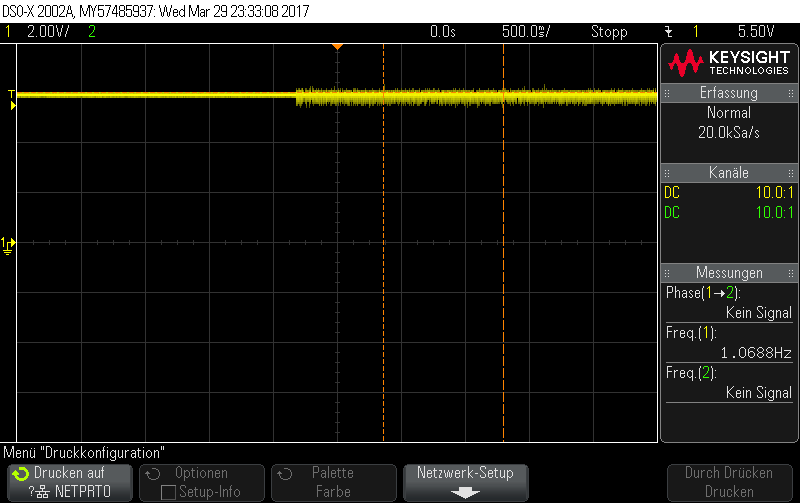
\includegraphics[width=\linewidth]{Messungen/Motor_Anschalten_rail.png}
		\caption{Motorrail beim Einschalten, Gesamtansicht}
	\end{minipage}
	\hfill
	\begin{minipage}{0.48\linewidth}
		\centering
		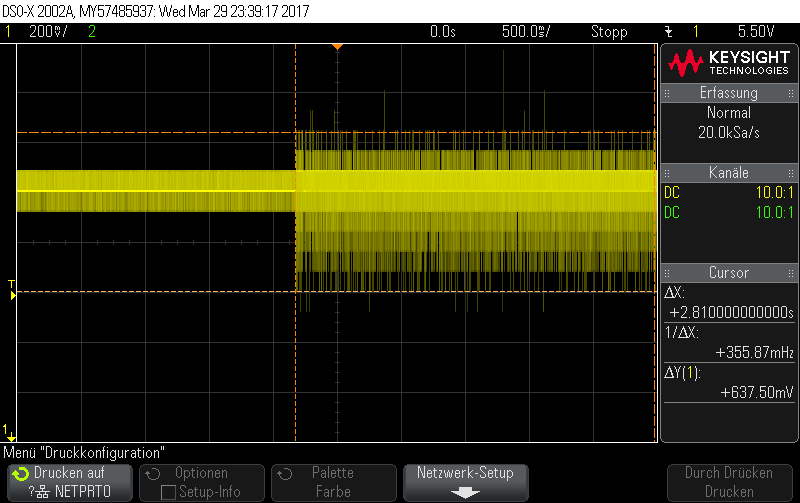
\includegraphics[width=\linewidth]{Messungen/Motor_rail_anschalten_zoom (1).png}
		\caption{Motorrail beim Einschalten, Zoomaufnahme}
	\end{minipage}
\end{figure}

In der Gesamtansicht ist zu erkennen, dass die Motorrail nach dem Einschalten auf ein Spannungsniveau von ungefähr 5,5\,V ansteigt. Nach dem Übergang bleibt die Versorgung grundsätzlich bestehen, auf der Spannung ist jedoch ein sichtbarer hochfrequenter Ripple überlagert. Die Zoomaufnahme zeigt den Einschaltmoment genauer. Dort ist erkennbar, dass die Spannung nicht völlig sprunghaft und ideal ansteigt, sondern von einem kurzzeitigen Stör- beziehungsweise Schwinganteil begleitet wird.

Aus der Cursoranzeige der Zoomaufnahme ergibt sich für den markierten Bereich ein Spannungsunterschied von ungefähr 637,5\,mV. Dieser Wert ist nicht als dauerhafter Spannungsfehler zu interpretieren, sondern beschreibt die Größenordnung des beobachteten Einschaltvorgangs im vergrößerten Ausschnitt. Kritische Einbrüche bis auf 0\,V oder ein offensichtliches vollständiges Zusammenbrechen der Motorrail sind in den gezeigten Aufnahmen nicht zu erkennen.

Für die praktische Bewertung bedeutet das: Die Motorrail schaltet grundsätzlich funktionsfähig ein, zeigt beim Übergang aber ein erkennbares Störverhalten, das bei empfindlicher Last oder bei gleichzeitigem Betrieb mehrerer Motoren weiter beobachtet werden sollte. Für eine endgültige Beurteilung wäre es sinnvoll, dieselbe Messung zusätzlich unter realer Motorlast und mit definiertem Einschaltstrom zu wiederholen. Damit ließe sich besser abschätzen, ob das beobachtete Verhalten lediglich normales Schaltwandler-Ripple ist oder ob im realen Betrieb zusätzliche Maßnahmen zur Entstörung notwendig werden.

\subsection{Messung an einem Encoder-Ausgang}
Die Encoder dienen als Rückführung für die spätere Motorregelung. In dieser Messung wurde nicht jeder Encoderanschluss einzeln geprüft, sondern ein Encoder-Ausgang exemplarisch untersucht.

\subsubsection{Messziel}
Bei der Encodermessung soll anhand eines einzelnen Encoder-Ausgangs überprüft werden,

\begin{itemize}
	\item ob die Signale elektrisch sauber und störungsarm vorliegen,
	\item ob die Impulsfolge zur tatsächlichen Bewegung passt,
	\item ob sich die Drehrichtung eindeutig erkennen lässt,
	\item ob die Auflösung und Genauigkeit für die geplante Regelung ausreichend sind.
\end{itemize}

\subsubsection{Messaufbau}
Ein Motor mit angeschlossenem Encoder wird kontrolliert betrieben. Gemessen wurde ein einzelner Encoder-Ausgang, bevor dessen Signale an die Zählereingänge des STM32 geführt werden. Dabei kann der Motor mit verschiedenen Drehzahlen und in beiden Drehrichtungen betrieben werden.

Zur Untersuchung eignen sich vor allem:

\begin{itemize}
	\item Oszilloskop zur Darstellung des gemessenen Encoder-Ausgangs
	\item Logikanalysator zur Impulszählung und Richtungsanalyse
	\item Vergleich mit einer bekannten mechanischen Bewegung oder Umdrehungszahl
\end{itemize}

Das Ergebnis soll sowohl elektrisch als auch funktional bewertet werden. Neben den Pegeln ist vor allem wichtig, ob die Flanken sauber erkennbar sind und ob die Drehrichtung aus Kanal A und Kanal B dieses einen Encoders abgeleitet werden kann. Die Messung steht damit exemplarisch für die übrigen gleich aufgebauten Encoderanschlüsse.

\begin{figure}[H]
	\centering
	\begin{tikzpicture}[font=\scriptsize, node distance=1.1cm, >=latex]
		\tikzstyle{block} = [draw, rectangle, rounded corners=2pt, minimum height=1.0cm, minimum width=2.2cm, align=center]
		\tikzstyle{signal} = [draw, rectangle, minimum height=0.65cm, minimum width=1.35cm, align=center]
		\tikzstyle{line} = [draw, -latex']

		\node[block, fill=red!10] (driver) {Motortreiber};
		\node[block, fill=green!12, right=1.6cm of driver] (motor) {DC-Motor\\mit Encoder};
		\node[signal, fill=yellow!20, right=1.35cm of motor, yshift=0.45cm] (a) {Encoder A};
		\node[signal, fill=yellow!20, below=0.2cm of a] (b) {Encoder B};
		\node[block, fill=purple!12, below=1.1cm of b, xshift=1.8cm] (scope) {Oszilloskop};
		\node[block, fill=blue!12, right=5cm of motor] (stm) {STM32\\Zählereingänge};
		
		\coordinate (tapA) at ($(a.east)!0.32!(stm.west |- a.east)$);
		\coordinate (tapB) at ($(b.east)!0.68!(stm.west |- b.east)$);
		\coordinate (ch1out) at ([xshift=-0.35cm]scope.north);
		\coordinate (ch2out) at ([xshift=0.35cm]scope.north);
		\coordinate (ch1mid) at (tapA |- ch1out);
		\coordinate (ch2mid) at (tapB |- ch2out);
		\coordinate (toplineL) at ([xshift=-0.35cm,yshift=0.85cm]driver.north west);
		\coordinate (toplineR) at ([xshift=0.35cm]stm.east |- toplineL);

		\draw[line] (driver) -- node[above] {Motorleitung} (motor);
		\draw[line] (motor.east) |- (a.west);
		\draw[line] (motor.east) |- (b.west);
		\draw[line] (stm.east) -- ++(0.35,0) |- (toplineR) -- (toplineL) |- (driver.west);
		\draw[line] (a.east) -- node[above] {A} (stm.west |- a.east);
		\draw[line] (b.east) -- node[above] {B} (stm.west |- b.east);
		\draw[draw] (ch1out) -| node[left, yshift=0.5cm] {CH1} (ch1mid) -- (tapA);
		\draw[draw] (ch2out) -| node[right, yshift=0.5cm] {CH2} (ch2mid) -- (tapB);
	\end{tikzpicture}
	\caption{Messaufbau zur Prüfung eines einzelnen Encoder-Ausgangs}
\end{figure}

Die folgenden Oszilloskopbilder zeigen den gemessenen Encoder-Ausgang bei konstanter halber Motorgeschwindigkeit in beide Richtungen. Kanal 1 ist orange dargestellt, Kanal 2 grün. Beide Kanäle wurden mit 1 V/div und derselben Zeitbasis aufgenommen, wodurch sich die Vorwärts- und Rückwärtsmessung direkt vergleichen lassen.

\begin{figure}[H]
	\centering
	\begin{minipage}{0.48\linewidth}
		\centering
		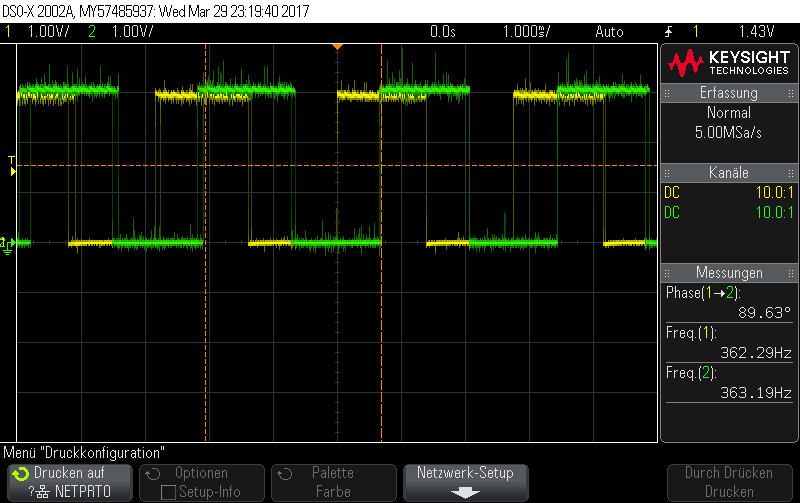
\includegraphics[width=\linewidth]{Messungen/vor_neuneu.png}
		\caption{Encoder-Ausgang bei Vorwärtsbewegung}
	\end{minipage}
	\hfill
	\begin{minipage}{0.48\linewidth}
		\centering
		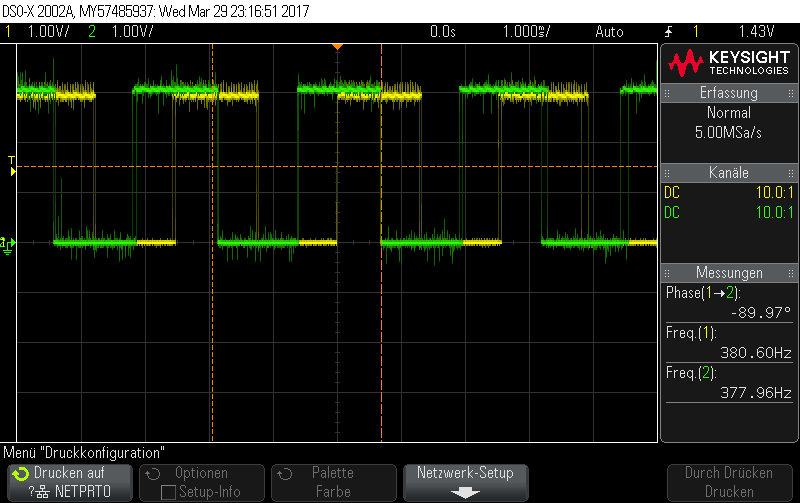
\includegraphics[width=\linewidth]{Messungen/rueck_neuneu.png}
		\caption{Encoder-Ausgang bei Rückwärtsbewegung}
	\end{minipage}
\end{figure}

\begin{table}[H]
	\centering
	\scriptsize
	\renewcommand{\arraystretch}{1.25}
	\setlength{\tabcolsep}{3pt}
	\begin{tabularx}{\linewidth}{L{0.17\linewidth}|L{0.14\linewidth}|L{0.14\linewidth}|L{0.16\linewidth}|L{0.23\linewidth}}
		\hline
		\textbf{Messpunkt} & \textbf{Pegel} & \textbf{Frequenz} & \textbf{Phasenlage} & \textbf{Bewertung} \\\hline
		Vorwärts, Kanal A/B & ca. 3 V$_{SS}$ & 362,23 Hz / 363,19 Hz & +89,63$^\circ$ & sauberes Quadratur-Signal bei konstanter halber Geschwindigkeit \\\hline
		Rückwärts, Kanal A/B & ca. 3 V$_{SS}$ & 380,60 Hz / 377,96 Hz & -89,97$^\circ$ & Quadratur-Signal plausibel, Richtung gegenüber Vorwärts invertiert \\\hline
	\end{tabularx}
	\caption{Messwerttabelle für den gemessenen Encoder-Ausgang}
\end{table}

\subsubsection{Messschaltung}
Die Signale des gemessenen Encoders werden über die dafür vorgesehenen Leitungen an den Mikrocontroller geführt. Für die Messung wurde dieser eine Encoder-Ausgang parallel an ein Oszilloskop oder einen Logikanalysator angeschlossen. Die übrigen Encoderanschlüsse wurden nicht einzeln vermessen.

\subsubsection{Auswertung und Interpretation}
Ausgewertet werden insbesondere Tastverhältnis, Signalpegel und Phasenlage der beiden Kanäle des gemessenen Encoder-Ausgangs. Die Phasenverschiebung zwischen den Kanälen gibt dabei Aufschluss über die Drehrichtung. Unscharfe Flanken, starke Störungen oder Pegelprobleme würden auf Schwachstellen in der Signalaufbereitung, Leitungsführung oder Pegelanpassung hinweisen.

Die neu aufgenommenen Signale zeigen das erwartete Verhalten eines Quadratursignals bei konstanter halber Motorgeschwindigkeit. In beiden Bildern sind zwei saubere Rechtecksignale mit nahezu gleicher Frequenz erkennbar. Für die Vorwärtsbewegung wurden 362,23 Hz auf Kanal 1 und 363,19 Hz auf Kanal 2 gemessen, bei einer Phasenlage von +89,63$^\circ$. Für die Rückwärtsbewegung wurden 380,60 Hz auf Kanal 1 und 377,96 Hz auf Kanal 2 mit einer Phasenlage von -89,97$^\circ$ gemessen. Damit liegt die Phasenverschiebung in beiden Fällen praktisch ideal bei 90$^\circ$ und das Vorzeichen der Phasenlage wechselt wie erwartet mit der Drehrichtung.

Gegenüber den früheren Aufnahmen sind diese Messungen deutlich belastbarer, weil Vorwärts- und Rückwärtsfahrt bei konstanter halber Geschwindigkeit aufgenommen wurden und das Oszilloskop in beiden Fällen numerische Werte für Frequenz und Phasenlage anzeigt. Kleine Frequenzabweichungen zwischen den beiden Drehrichtungen sind bei manuell eingestellter Geschwindigkeit plausibel und ändern nichts an der grundsätzlichen Aussage. Die Messung zeigt damit, dass der Encoder elektrisch saubere Signale liefert und dass der STM32 die Flanken für eine spätere Richtungs- und Drehzahlauswertung grundsätzlich zuverlässig erfassen kann.

\subsection{Messungen an Motoren und Servos}
Die dritte im Antrag vorgesehene Messgruppe betrifft die Leistungsaufnahme und die Funktion von Motoren und Servos unter Last. Die grundsätzliche Stabilität der Powerrails wurde bereits in Abschnitt 9.1 betrachtet. Hier geht es daher um den realen Betrieb der Aktoren: Wie viel Strom beziehungsweise Leistung wird benötigt und funktioniert die Ansteuerung auch unter Belastung zuverlässig.

\subsubsection{Messziel}
Mit diesen Messungen soll untersucht werden,

\begin{itemize}
	\item wie groß die Stromaufnahme der Motoren und Servos im Leerlauf und unter Last ist,
	\item welche Leistung im praktischen Betrieb benötigt wird,
	\item ob Motoren und Servos bei der jeweiligen Last korrekt funktionieren.
\end{itemize}

\subsubsection{Messaufbau}
Ein Motor beziehungsweise Servo wird an die reale Ausgangsstufe des Boards angeschlossen und anschließend in mehreren Betriebsfällen untersucht. Sinnvolle Lastfälle sind beispielsweise:

\begin{itemize}
	\item Leerlaufbetrieb
	\item Anlaufmoment
	\item Betrieb unter mechanischer Last
	\item blockierter oder nahezu blockierter Zustand für kurze kontrollierte Zeit
\end{itemize}

Gemessen werden dabei Strom und Spannung am jeweiligen Aktor beziehungsweise an dessen Versorgung. Daraus kann die Leistungsaufnahme berechnet werden. Zusätzlich wird die Funktion unter Last beurteilt, also ob Motor oder Servo die gewünschte Bewegung ausführen und ob es zu Aussetzern, starkem Einbruch der Versorgung oder auffälliger Erwärmung kommt.

Die Messwerte sollen getrennt nach Motoren und Servos dokumentiert werden. Dadurch lässt sich später erkennen, ob die Aktoren und deren Ansteuerung für die geplante Belastung ausreichend dimensioniert sind.

\begin{figure}[H]
	\centering
	\begin{tikzpicture}[font=\scriptsize, node distance=1.05cm, >=latex]
		\tikzstyle{block} = [draw, rectangle, rounded corners=2pt, minimum height=1.0cm, minimum width=2.25cm, align=center]
		\tikzstyle{meter} = [draw, circle, minimum size=0.75cm, align=center]
		\tikzstyle{line} = [draw, -latex']

		\node[block, fill=blue!12] (board) {Controller \\ STM32/PI};
		\node[block, fill=red!10, right=1.5cm of board] (stage) {Treiberstufe\\oder Servoport};
		\node[meter, fill=yellow!20, right=1.15cm of stage] (amp) {A};
		\node[block, fill=green!12, right=1.15cm of amp] (load) {Motor\\oder Servo};
		\node[block, fill=purple!12, below=1.05cm of amp] (scope) {Oszilloskop};
		\coordinate (out) at ($(stage.east)!0.5!(amp.west)$);
		\coordinate (gndL) at ([yshift=-1.45cm]stage.south west);
		\coordinate (gndR) at ([yshift=-1.45cm]load.south east);

		\draw[line] (board) -- node[above] {PWM / I\textsuperscript{2}C} (stage);
		\draw[line] (stage) -- (amp);
		\draw[line] (amp) -- node[above] {Laststrom} (load);
		\draw[draw] (gndL) -- node[below] {GND} (gndR);
		\draw[draw] (load.south) -- (load.south |- gndL);
		\draw[draw] ([xshift=-0.32cm]scope.north) |- node[left, yshift=0.35cm] {Signal} (out);
		\draw[draw] ([xshift=0.32cm]scope.south) |- node[right, yshift=-0.25cm] {GND} (scope.south |- gndL);
	\end{tikzpicture}
	\caption{Messaufbau für Motor- und Servomessungen}
\end{figure}

\begin{table}[H]
	\centering
	\scriptsize
	\renewcommand{\arraystretch}{1.25}
	\setlength{\tabcolsep}{3pt}
	\begin{tabularx}{\linewidth}{L{0.15\linewidth}|L{0.15\linewidth}|L{0.12\linewidth}|L{0.12\linewidth}|L{0.13\linewidth}|L{0.16\linewidth}}
		\hline
		\textbf{Verbraucher} & \textbf{Lastfall} & \textbf{Spannung} & \textbf{Strom} & \textbf{Leistung} & \textbf{Funktion unter Last} \\\hline
		DC-Motor & Leerlauf &  &  &  &  \\\hline
		DC-Motor & Anlauf &  &  &  &  \\\hline
		DC-Motor & Last &  &  &  &  \\\hline
		Servo & Ruheposition &  &  &  &  \\\hline
		Servo & Bewegung &  &  &  &  \\\hline
		Servo & Last &  &  &  &  \\\hline
	\end{tabularx}
	\caption{Vorgesehene Messwerttabelle für Motoren und Servos}
\end{table}

\subsubsection{Messschaltung}
Die Strommessung erfolgt über ein in Serie geschaltetes Messgerät oder über einen Shunt. Die Spannung wird an der Versorgung des jeweiligen Aktors gemessen. Bei Motoren ist dafür die Motorrail im realen Motorbetrieb relevant, bei Servos die Servo-Rail direkt am Servo oder an der Servo-Versorgung. Die Leistung wird anschließend aus Spannung und Strom berechnet.

Das Oszilloskop kann zusätzlich verwendet werden, um das PWM-Signal oder kurze Spannungseinbrüche sichtbar zu machen. Für die eigentliche Messaufgabe reichen jedoch vor allem die Leistungsaufnahme und die Beobachtung, ob der Aktor unter Last korrekt arbeitet.

\subsubsection{Auswertung und Interpretation}
Die Auswertung beschränkt sich auf die Leistungsaufnahme und die Funktion unter Last. Dazu werden Spannung, Strom und daraus die Leistung betrachtet. Zusätzlich wird bewertet, ob Motoren und Servos die gewünschte Bewegung ausführen, ob die Versorgung dabei stark einbricht und ob Treiber oder Aktoren auffällig warm werden. Damit wird geprüft, ob die Aktoren im geplanten Einsatzbereich zuverlässig betrieben werden können.

